\documentclass[10pt]{article}

% --- packages -------------------------------------------------------------
\usepackage[T1]{fontenc}
\usepackage[utf8]{inputenc}
\usepackage{lmodern}
\usepackage[a4paper,margin=0.72in]{geometry}
\usepackage{microtype}
\usepackage{amsmath,amssymb}
\usepackage{booktabs}
\usepackage{graphicx}
\usepackage{caption}
\usepackage{enumitem}
\usepackage{siunitx}
\usepackage{xcolor}
\usepackage{titlesec}
\usepackage{multicol}
\usepackage{tcolorbox}
\usepackage[hidelinks]{hyperref}

% --- style ----------------------------------------------------------------
\definecolor{vblue}{HTML}{1F4E79}
\definecolor{vlight}{HTML}{EAF0F6}
\definecolor{vgray}{HTML}{5A6470}
\hypersetup{colorlinks=true, linkcolor=vblue, urlcolor=vblue, citecolor=vblue}
\captionsetup{font=footnotesize,labelfont=bf,labelsep=period}
\setlist{itemsep=1pt,topsep=2pt,parsep=0pt,leftmargin=1.1em}
\sisetup{detect-all,group-minimum-digits=4}
\pagestyle{empty}

\titleformat{\section}{\normalsize\bfseries\color{vblue}}{}{0em}{}
\titlespacing{\section}{0pt}{6pt}{2pt}

\newcommand{\Cllr}{C_{\mathrm{llr}}}
\newcommand{\code}[1]{\texttt{\small #1}}

% Boxed callout for the headline claim.
\newtcolorbox{claimbox}{
  colback=vlight, colframe=vblue, boxrule=0.6pt, arc=2pt,
  left=8pt, right=8pt, top=5pt, bottom=5pt
}

\begin{document}

% ---- masthead ------------------------------------------------------------
{\LARGE\bfseries Verity}\hfill{\color{vgray}\small Executive Capability Brief \;\textbar\; June 2026}\\[2pt]
{\color{vblue}\rule{\linewidth}{1.2pt}}\\[3pt]
{\large A calibrated, auditable deployment layer for forensic surface comparison}\\[2pt]
{\color{vgray}\small Eric Hare \;\textbar\; \href{mailto:ericrhare@gmail.com}{ericrhare@gmail.com}}

\vspace{4pt}
\begin{claimbox}
\textbf{The thesis.} Verity is not a new matching algorithm. It is the
\textbf{production, calibration, and validation layer} for the CSAFE / Iowa State
research program (Hare, Hofmann \& Carriquiry 2017) and the NIST congruent-matching
line (Song 2013). It reports a \textbf{calibrated weight of evidence} (a likelihood
ratio) with a \textbf{characterized cost} ($\Cllr$) on a \textbf{named} reference
population --- and refuses to emit an answer outside the domain it was validated on.
It does \emph{not} claim a universal error rate, because none exists.
\end{claimbox}

\vspace{2pt}
% ---- the problem ---------------------------------------------------------
\section{The problem}
The NRC (2009) and PCAST (2016) reports found that feature-comparison forensic
disciplines --- firearms and toolmarks among them --- lack \emph{characterized error
rates}. Cuellar et al.\ (2024) went further: \emph{no} black-box study of firearm
comparison has properly characterized one, largely because studies test on the same
sources they were tuned on and report study-specific numbers as if they were
properties of the whole discipline. The field needs a defensible, reproducible way
to state how strong firearm/toolmark evidence is --- one that survives scrutiny.

% ---- the answer ----------------------------------------------------------
\section{Verity's answer}
\begin{itemize}
  \item \textbf{Report a likelihood ratio, not a verdict.} How much more probable the
        observed surface agreement is under same-source than different-source ---
        prior-independent, the form courts and statisticians ask for.
  \item \textbf{Characterize it honestly.} Quote the calibration cost $\Cllr$
        (Br\"ummer \& du Preez 2006) measured \emph{source-disjoint} (no firearm in
        both training and test), reported \emph{per study} --- never pooled across
        makes for error-rate claims.
  \item \textbf{Know your limits.} An applicability-domain gate declines to score a
        scan outside the validated domain instead of extrapolating.
\end{itemize}

% ---- what's novel --------------------------------------------------------
\section{What is genuinely new (and what is borrowed)}
\begin{multicols}{2}
\textbf{Built on (credited):} the CSAFE bullet-matching method and
\code{bulletxtrctr}; Song's Congruent Matching Cells for cartridge cases; the
Chumbley toolmark statistic; the ISO~25178-72 X3P format and \code{x3ptools}; the
$\Cllr$ metric from forensic speaker recognition.

\columnbreak

\textbf{New in Verity:}
\begin{enumerate}[leftmargin=1.3em]
  \item \textbf{Unification} via \emph{Congruent Matching Regions} --- one algorithm
        across striated, impressed, and fractured marks.
  \item A \textbf{calibrated-LR answer} to Cuellar et al.
  \item A \textbf{glass-box} decision layer: region attribution + an
        \emph{audit firewall}.
  \item \textbf{Production engineering}: native Rust X3P codec, deployed API.
  \item A \textbf{data-selected scorer} ($\code{diag\_contrast}$).
\end{enumerate}
\end{multicols}

% ---- how it works --------------------------------------------------------
\section{How it works}
\textbf{One pipeline, any mark.} ISO-standard surface metrology (degree-2 form
removal; ISO~16610 roughness band, $\lambda_s=\SI{4}{\micro\meter}$,
$\lambda_c=\SI{250}{\micro\meter}$) $\rightarrow$ FFT-based striae orientation and
signature extraction $\rightarrow$ comparison $\rightarrow$ a calibrated likelihood
ratio. \textbf{Congruent Matching Regions} generalizes Song's cell-counting:
partition one surface into regions, register each against the other, count the
regions whose best-fit transforms agree. A 1-D window under lag parallels the
Chumbley striae statistic; a 2-D cell under translation+rotation instantiates CMC; a
3-D patch handles fractures. \textbf{The audit firewall} turns any score into an LR
through a \emph{monotone, bounded} calibration (Platt scaling, capped at what the
reference supports, with a bootstrap interval) --- so the evidence is
interpretable no matter how the score was produced, and the system reports
\emph{which regions} drove the match.

% ---- evidence ------------------------------------------------------------
\section{The evidence}
On the Hamby-252 consecutively-rifled benchmark, under the source-disjoint protocol
that directly answers Cuellar et al.:

\begin{claimbox}
\centering
\textbf{Barrel-disjoint test $\Cllr = \num{0.113}\pm\num{0.066}$ \quad\textbar\quad
test AUC $= \num{1.000}\pm\num{0.001}$}\\[1pt]
{\small (full-study totals: 46 same-source / 549 different-source pairs across 10
barrels; each fold tests only the pairs among its four held-out barrels; in-sample
$\Cllr = \num{0.077}$, $\Cllr^{\min}=\num{0.032}$, ECE $=\num{0.031}$,
EER $=\SI{2.1}{\percent}$.)}
\end{claimbox}

\vspace{3pt}
\begin{minipage}[t]{0.5\linewidth}
  \centering
  \captionof{table}{Source-disjoint test $\Cllr$ per study (lower is better);
    \textbf{bold} = better scorer. Reported per study, never pooled.}
  \footnotesize
  \begin{tabular}{@{}lcc@{}}
    \toprule
    \textbf{Study} & \textbf{\code{diag\_mean}} & \textbf{\code{diag\_contrast}} \\
    \midrule
    Hamby-252      & \num{0.121} & \textbf{\num{0.113}} \\
    PGPD Beretta   & \num{0.299} & \textbf{\num{0.273}} \\
    Phoenix Ruger  & \textbf{\num{0.252}} & \num{0.354} \\
    Hamby-173      & \num{0.456} & \textbf{\num{0.338}} \\
    \bottomrule
  \end{tabular}
\end{minipage}\hfill
\begin{minipage}[t]{0.46\linewidth}
  \centering
  \vspace{-2pt}
  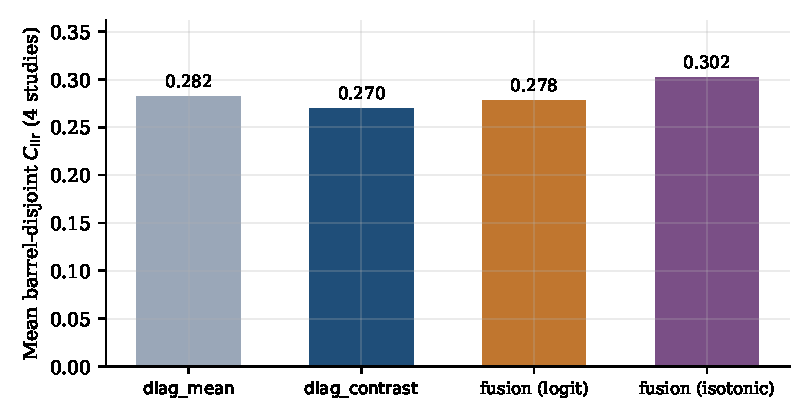
\includegraphics[width=\linewidth]{fig_scorer_selection.pdf}
  \captionof{figure}{Scorer chosen \emph{by data}: \code{diag\_contrast} has the
    lowest cross-study source-disjoint $\Cllr$; adding fusion capacity does not help,
    and the isotonic fusion overfits.}
\end{minipage}

\vspace{4pt}
% ---- platform + scope ----------------------------------------------------
\begin{multicols}{2}
\section{The platform}
\begin{itemize}
  \item Native \textbf{Rust X3P codec} (ISO~25178-72) with Python \& R bindings ---
        fast, dependency-light, interoperable with \code{x3ptools}.
  \item A \textbf{deployed calibrated-LR REST API}: \code{/detect}, \code{/compare}
        (bounded LR + credible interval + region attribution), \code{/health}
        (publishes the calibrated domains).
  \item A \textbf{data catalog} that harvests/labels the open NBTRD 3-D scans, and a
        \textbf{reproducible validation harness} behind every number here.
\end{itemize}

\columnbreak

\section{Honest scope}
\begin{itemize}
  \item The scorer and front-end were selected on the same four studies reported
        here; a one-shot confirmation on untouched data is the next milestone.
  \item Consecutively-manufactured benchmarks are small in \emph{sources}
        (8--10 barrels; Fadul $\approx\!10$ slides), so fold-to-fold $\Cllr$ varies.
  \item A score-based LR is a property of the score and the named reference, not an
        unconditional measure --- hence the scope gate.
  \item \textbf{No universal error rate} is claimed; every number is conditioned on a
        named population and a stated protocol.
  \item The learned (Phase-2b) representation does not yet beat the interpretable
        baseline; the baseline is deployed.
\end{itemize}
\end{multicols}

\vspace{2pt}
{\color{vblue}\rule{\linewidth}{0.6pt}}\\[2pt]
{\footnotesize\color{vgray}\textbf{An invitation, not a claim of endorsement.}
Verity is the deployment and calibration layer for a research program it did not
invent. The next step is validation on larger, representative, genuinely
source-disjoint references --- the data the CSAFE program is built to produce. The
codec, the calibration firewall, and the validation harness are offered as open
infrastructure for that collaboration. Mention of CSAFE, Iowa State, or NIST denotes
intellectual lineage and a prospective partnership only; it does not imply review or
endorsement.}

\end{document}
